\documentclass[preprint,12pt,a4paper]{elsarticle}

% JISA-oriented Elsevier initial-submission source.
% Single-column preprint layout; numerical references; editable tables and vector figures.
\usepackage[T1]{fontenc}
\usepackage{lmodern}
\usepackage[utf8]{inputenc}
\usepackage{amsmath,amssymb,amsthm,mathtools}
\usepackage{booktabs,tabularx,array,multirow,makecell}
\newcolumntype{Y}{>{\raggedright\arraybackslash}X}
\usepackage{siunitx}
\usepackage{graphicx}
\usepackage{xcolor}
\usepackage{tikz}
\usetikzlibrary{arrows.meta,positioning,calc,fit,shapes.geometric,patterns,matrix}
\usepackage{pgfplots}
\usepgfplotslibrary{groupplots}
\pgfplotsset{compat=1.18}
\usepackage{enumitem}
\usepackage{url}
\usepackage{xspace}
\usepackage[hidelinks]{hyperref}
\usepackage[nameinlink,noabbrev]{cleveref}

\journal{Journal of Information Security and Applications}

\newtheorem{proposition}{Proposition}
\newtheorem{corollary}{Corollary}
\newcommand{\ProposedSystem}{the proposed system\xspace}
\newcommand{\RDHEI}{\textsc{RDHEI}\xspace}
\newcommand{\RRBE}{\textsc{RRBE}\xspace}
\newcommand{\bpp}{\text{bpp}}
\newcommand{\Linf}{\ell_{\infty}}
\newcommand{\Kauth}{K_{\mathrm{auth}}}
\newcommand{\Kimg}{K_{\mathrm{img}}}
\newcommand{\Kh}{K_{\mathrm{h}}}
\newcommand{\Nnet}{N_{\mathrm{net}}}
\newcommand{\Ggross}{G_0}
\newcommand{\Fboot}{F}
\newcommand{\Bback}{B}
\newcommand{\Hboot}{H}
\newcommand{\Savail}{S}
\sisetup{detect-all,group-separator={,},group-minimum-digits=4}
\setlength{\emergencystretch}{3em}

\begin{document}

\begin{frontmatter}

\title{Context-invariant prediction and authenticated phase discovery for reversible data hiding in encrypted images}

\author[inst1]{[Author name]}
\ead{[Corresponding author email]}
\author[inst1]{[Co-author name]}
\address[inst1]{[Department, institution, city, country]}

\begin{abstract}
Prediction-based reversible data hiding in encrypted images (RDHEI) requires the prediction inputs used during embedding and recovery to remain identical after carrier modification. We present EDR2, a reserve-room-before-encryption protocol for native 8-bit grayscale images using a frozen residual CNN with centre-masked $3\times3$ input patches. Carrier centres are restricted to one of four step-2 lattice phases. Because each candidate centre is masked and distinct selected centres are separated by at least two pixels in Chebyshev distance, writes to selected centres do not alter any candidate's predictor input. The content owner evaluates all four phases and selects the one with maximum signed net payload after accounting for the compressed label directory, bootstrap-carrier opportunity cost and backup of original bootstrap bytes. HKDF-derived keys, AES-256-CTR and HMAC-SHA256 protect the image and in-band packet; the receiver discovers the selected phase without per-image sidecar metadata. On 243 hash-verified native 8-bit grayscale USC-SIPI images, 163/243 produced positive net capacity and all 978 receiver trials on this accepted subset recovered both host and payload exactly. Mean per-image and pooled usable rates were 0.1432 and 0.0955 bpp. Same-corpus native-protocol reproductions of Multi-MSB+Huffman and corrected PPMR achieved higher rates, while a separate matched-grid study found that a $5\times5$ no-weighted-loss CNN ablation outperformed the selected $3\times3$ predictor in MAE and positive-net coverage. EDR2 is therefore evaluated as a specific prediction-synchronization and authenticated-recovery construction, not as a capacity-superior RDHEI method.

\end{abstract}

\begin{keyword}
reversible data hiding \sep encrypted images \sep prediction invariance \sep authenticated metadata \sep exact recovery \sep multimedia security
\end{keyword}

\end{frontmatter}

\section{Introduction}
\label{sec:intro}

Reversible data hiding (RDH) embeds an auxiliary message in a host signal while preserving the ability to reconstruct the original host exactly after extraction. In encrypted-image RDH, confidentiality must be maintained while the data hider works on an encrypted representation. A common system separates three roles: the content owner prepares and encrypts the image, an independent hider inserts the user payload, and an authorised receiver extracts the payload and reconstructs the original image. The reserve-room-before-encryption (\RRBE) architecture creates embedding room while the image is still available to the owner, then allows the hider to insert data after encryption \cite{zhang2011,ma2013,puteaux2021survey}.

Prediction-based schemes exploit spatial redundancy in the plaintext image. A predictor estimates a candidate pixel from its neighbours; the prediction error determines how many most-significant bits (MSBs) can be replaced while retaining enough information for exact recovery. Learned predictors, including CNN-based predictors, have also been used in RDHEI \cite{ping2024,cheng2025masked}. However, an encoder and decoder that use the same checkpoint can still disagree if embedding changes samples in the predictor's receptive field. The relevant requirement is not merely shared weights: it is that the prediction inputs used during preparation and recovery remain compatible.

This paper studies a concrete spatial condition for a fixed centre-masked $3\times3$ CNN predictor. Only centres on one selected step-2 phase may be modified. Every pair of distinct centres in that phase is separated by at least two pixels in the Chebyshev metric, while the value at the candidate centre is masked before inference. Hence, no other mutable candidate is inside the $3\times3$ patch, and the candidate's own value is hidden from the predictor. The resulting proposition guarantees equality of the masked predictor inputs before and after arbitrary writes to the selected carrier centres, subject to the stated fixed inference procedure.

Four phases provide equal geometric candidate density but can produce different prediction labels, compressed directory lengths and bootstrap opportunity costs. The owner therefore evaluates all four phases independently and chooses the phase with the highest signed net payload. The phase is not sent as an external field: the receiver tests the four public header locations and accepts exactly one location whose framing, phase-bound HMAC and bounded directory validation succeed. All image-dependent recovery information, including the encrypted header, compressed label directory, authentication tag and bootstrap-byte backup, is stored in the marked encrypted image.

The aim is deliberately not to present \ProposedSystem as a high-capacity alternative to recent RDHEI methods. On the evaluated corpus, its usable rates are much lower than those of two reproduced external implementations and than several rates reported in recent JISA papers. The paper instead evaluates a narrow synchronisation condition, the exact-recovery contract that uses it, the gain from phase selection, and the full cost of in-band recovery metadata. The empirical comparison is reported without suppressing the negative-capacity images or the weaker predictor ablation.

The paper makes four bounded contributions:
\begin{enumerate}[leftmargin=*,itemsep=2pt]
\item A formal input-invariance proposition for a frozen, centre-masked radius-one predictor when all mutable carrier centres in a phase are pairwise Chebyshev-separated by at least two.
\item A four-phase maximum-density candidate construction and a deterministic rule that selects the phase with the greatest signed net payload after directory and bootstrap costs.
\item An encrypted in-band packet in which the candidate phase is inferred from the authenticated header location; the receiver's per-image semantic inputs are the marked encrypted image, a 32-byte master key and a 128-bit nonce.
\item A reproducible evaluation on 243 native grayscale images, including phase ablation, predictor comparisons, native-protocol external reproductions, exact-recovery trials, parser robustness and runtime measurements.
\end{enumerate}

The claims have important boundaries. Checkerboard sampling, MSB replacement, prediction-error coding, CNN prediction for RDHEI, masked image prediction, compressed auxiliary maps, authenticated RDHEI and adaptive block selection have prior art \cite{yi2018,puteaux2018,yin2020,yin2021,ren2023,sui2023,ping2024,ren2025auth,ankur2025,huang2025bfe,ren2026abpde}. The proposed system does not claim any of these as independently new. Nor does it claim a formal cryptographic proof, independent cryptographic certification, resistance to a malicious authorised hider, or state-of-the-art capacity.

\section{Related work}
\label{sec:related}

\subsection{RDH and encrypted-image architectures}

Zhang's early encrypted-image RDH construction established that data can be embedded in an encrypted image while preserving reversibility \cite{zhang2011}. Ma et al. developed the RRBE architecture in which reversible room is prepared before encryption and subsequently used by an independent hider \cite{ma2013}. Surveys by Shi et al. and Puteaux et al. describe the broader RDH and RDHEI design space, including encryption order, receiver capabilities and recovery side information \cite{shi2016,puteaux2021survey}. These distinctions matter when comparing rates: a reported bpp value depends on the method's definition of payload, whether auxiliary data are charged, and whether host reconstruction is exact.

\subsection{Prediction, checkerboard sampling and MSB coding}

Prediction and MSB replacement are established RDHEI mechanisms. Yi and Zhou's checkerboard-based adaptive prediction partitions the image into reference and embeddable positions \cite{yi2018}. Puteaux and Puech use MSB prediction to reserve capacity \cite{puteaux2018}. Yin et al. combine multi-MSB prediction with Huffman coding, and later propose pixel prediction with multi-MSB-plane rearrangement (PPMR) \cite{yin2020,yin2021}. Multi-prediction and hybrid prediction with Huffman-coded labels are also studied by Ren et al. and Sui et al. \cite{ren2023,sui2023}. Thus, the use of a spatial partition, the prediction of MSBs, and compression of a location/label representation are not new in isolation.

\subsection{Learned and masked predictors}

Ping et al. introduce an asymmetric CNN-based predictor and an adaptive-mean second stage for RDHEI \cite{ping2024}. Cheng et al. use a pixel-level masked autoencoder with polar coding \cite{cheng2025masked}. These works preclude a broad novelty claim based on either CNN use or masking. Adjacent JISA work in plaintext-domain RDH also uses a lightweight CNN to classify pixels and guide adaptive selection between classical predictors in a PVO-based flexible-strip scheme; that work is not an encrypted-image protocol, but it reinforces that CNN-guided adaptive prediction is established journal prior art \cite{fan2026cnn}. The narrower question addressed here is whether a fixed local predictor can be given a carrier geometry that guarantees unchanged per-candidate predictor inputs after the carrier-centre values are altered. The $3\times3$ centre-masked construction provides one specific answer; it is not a general claim about all masked predictors or all receptive-field shapes.

\subsection{Authentication and recovery integrity}

Ren et al. combine prediction-error compression with image and ciphertext authentication in RDHEI \cite{ren2025auth}. This is particularly relevant because it demonstrates that authentication is already part of the RDHEI literature. The proposed system uses HKDF-derived subkeys, AES-256-CTR and HMAC-SHA256 in its packet implementation. These standard cryptographic mechanisms are not claimed as new. AES-CTR does not itself provide integrity; the HMAC is a separate packet-authentication layer. The authenticated hider key is held by the authorised data hider, so a malicious authorised hider is outside the present threat model.

\subsection{Recent JISA RDHEI methods}

Recent JISA papers are especially important to the intended venue positioning. Ankur et al. use a hybrid predictor and bit-plane label maps with an optimal block-size encoding strategy, reporting 3.8770/3.9036 bpp on BOSSBase and 3.7944/3.8431 bpp on BOWS-2 for its Direct Bit-Stream (DBS)/Arithmetic Encoded Bit-Stream (AEBS) variants \cite{ankur2025}. Huang et al. combine a hybrid predictor, stream-cipher encryption, block scrambling and bidirectional flag encoding, reporting 3.76 and 3.37 bpp on the same datasets \cite{huang2025bfe}. Ren et al.'s adaptive block-level pixel-difference encoding (ABPDE) retains local redundancy through block modulation/permutation, codes pixel differences with adaptive Huffman coding, and reports average rates of 2.4938 bpp on BOSSBase and 2.3508 bpp on BOWS-2, at least 0.2845 and 0.2900 bpp above its compared methods, respectively \cite{ren2026abpde}. Gao and Gao combine multiple linear regression, multi-bit prediction and an adaptive Huffman-coded location map \cite{gao2025mlr}. Kim et al.'s pixel-shifting approach embeds four bits per block through encrypted-block permutation rather than MSB substitution \cite{kim2024psa}. Other JISA contributions include key-controlled balanced Huffman coding, 2D label/block classification, and redundancy-free cipher pixel rotation with multi-MSB replacement \cite{yang2024kbhc,yang2024label,qu2025rotation}.

The rates quoted above are taken from the respective papers' own descriptions. They are not controlled comparisons with \ProposedSystem: the datasets, encryption orders, carrier constructions and net-rate definitions differ. Nevertheless, the gap is material and must be acknowledged. Recent JISA work by Gao et al. combines exploiting modification direction with polynomial-based secret image sharing in two threshold RDHEI constructions. The EMD-RDHP variant is reported to reach up to 2 bpp but does not provide lossless recovery; a modified variant records modification operations to enable lossless reconstruction, although its separate rate is not isolated in the accessible abstract \cite{gao2026emd}. This work differs from the proposed system in its multi-share fault-tolerant threat model and separable recovery objective.



Other recent studies extend the design space beyond the direct JISA comparators. They include adaptive bit-plane classification with group coding, dual-stage bit-plane compression with CP-ABE recovery authorisation, D4-symmetry pixel shifting with context-aware recovery and in-band location maps, overlapping-block/shared-MSB coding, dynamic horizontal/vertical block partitions, texture-adaptive prediction and pixel classification, cross-domain neural prediction with divisor secret sharing, and key-controlled per-block embedding for telemedicine images \cite{zhou2026bitplane,peng2026,hung2026d4,tram2026,lin2026,wang2026apvcpc,shi2026neural,muhudin2026}. These approaches use different carrier families, threat models, key distribution and datasets; they establish relevant prior art but do not provide a harmonised capacity ranking against the proposed system.

The JISA comparisons sharpen the publication risk: even where the rate definitions cannot be equated, the proposed system's 0.0955 pooled usable bpp is far below the native rates reported by several recent methods. The present work must therefore stand on the specific synchronization and receiver-contract contribution and on rigorous empirical evidence, not on a capacity-superiority narrative.

\subsection{Novelty boundary and research question}

The narrow research question is: under what spatial condition do arbitrary writes to selected carrier centres leave every input patch of a fixed centre-masked radius-one predictor unchanged, and how can the phase be located by the receiver without per-image sidecar metadata? The proposed system provides a proof for one fixed $3\times3$ predictor and four step-2 phases. The signed-net phase selection and authenticated packet are necessary parts of the implemented composition, not claims of independently unprecedented adaptive partitioning, in-band metadata or authentication.

\section{System model and protocol requirements}
\label{sec:model}

\subsection{Parties and per-image information}

Let the original image be $X\in\{0,\ldots,255\}^{H\times W}$, with even $H$ and $W$ and native 8-bit grayscale samples. The content owner holds $X$, a 32-byte master key $K$, a 128-bit nonce $V$ that must be unique under $K$, and the preinstalled frozen CNN checkpoint. The owner prepares reversible room and encrypts the reserved image. The owner then provides the independent hider with the reserved encrypted image and a nonce-specific data-hiding capability key $\Kh$ over an assumed authenticated confidential key-delivery channel. The hider additionally receives the user payload. The hider does not receive the plaintext image or image-encryption key. The receiver's only per-image semantic inputs are the final marked encrypted image, $K$ and $V$; the decoder, fixed constants and checkpoint are shared installed software.

The design is therefore receiver-side free of external image-dependent sidecars. It does not claim that no key handoff occurs between owner and hider. The owner-to-hider capability is cryptographic key material, not a prediction map, label map or per-image recovery file.

\subsection{Security assumptions}

The image and data-hiding keys are derived through HKDF-SHA256 with distinct context strings. AES-256-CTR encrypts the image, header stages, directory and payload under separate derived keys. HMAC-SHA256 authenticates the marked packet, binding the image dimensions and the selected lattice phase as well as the marked image bytes (with the tag carrier bytes zeroed for MAC computation). The receiver verifies the tag before decrypting or decompressing the label directory and before CNN inference.

The protocol assumes nonce uniqueness under a master key. Reusing a nonce repeats derived keys and CTR keystreams and is prohibited. AES-CTR is a confidentiality transform, not an integrity mode; packet integrity is provided by the separate HMAC. The data hider possesses the authentication capability and can recompute a valid tag. Accordingly, the proposed system does not claim resistance to a malicious authorised hider. The owner-to-hider key-delivery channel is assumed confidential and authenticated. These are implementation assumptions, not a formal cryptographic proof.

\section{Proposed System}
\label{sec:method}

\begin{figure}[t]
\centering
\resizebox{\textwidth}{!}{%
\begin{tikzpicture}[
  x=1cm,y=1cm,>=Latex,font=\scriptsize,
  flow/.style={-{Latex[length=2mm]},thick,draw=black!75},
  panel/.style={draw=black!65,dashed,rounded corners=1.5mm,thick},
  owner/.style={draw=blue!55!black,fill=blue!5,rounded corners=2mm,thick,
    text width=1.42cm,minimum height=1.15cm,align=center,inner sep=3pt},
  ownerwide/.style={owner,text width=1.62cm},
  cnn/.style={draw=blue!65!black,fill=blue!8,rounded corners=2mm,thick,
    text width=1.45cm,minimum height=1.15cm,align=center,inner sep=3pt},
  select/.style={draw=orange!75!black,fill=yellow!16,rounded corners=2mm,thick,
    text width=1.25cm,minimum height=1.15cm,align=center,inner sep=3pt},
  hider/.style={draw=green!45!black,fill=green!7,rounded corners=2mm,thick,
    text width=2.30cm,minimum height=1.28cm,align=center,inner sep=4pt},
  receiver/.style={draw=violet!65!black,fill=violet!6,rounded corners=2mm,thick,
    text width=1.85cm,minimum height=1.20cm,align=center,inner sep=3pt},
  receiverwide/.style={receiver,text width=2.20cm},
  neutral/.style={draw=black!55,fill=black!3,rounded corners=2mm,thick,
    text width=1.75cm,minimum height=1.20cm,align=center,inner sep=3pt},
  roleowner/.style={draw=blue!30,fill=blue!10,rounded corners=2mm,thick,
    minimum height=0.42cm,align=center,font=\small\bfseries},
  rolehider/.style={draw=green!30!black,fill=green!10,rounded corners=2mm,thick,
    minimum height=0.42cm,align=center,font=\small\bfseries}
]
% (a) Content-owner reservation and encrypted-domain data hiding.
\draw[panel] (-0.25,0.05) rectangle (18.25,3.95);
\node[anchor=west,font=\small\bfseries] at (-0.02,3.72)
  {(a) Embedding process (content owner and independent data hider)};
\node[roleowner,minimum width=12.55cm] at (6.25,3.22)
  {Content owner: reserve room before encryption (RRBE)};
\node[rolehider,minimum width=5.05cm] at (15.55,3.22)
  {Independent data hider: encrypted domain};

\node[owner] (plain) at (0.78,1.68)
  {\textbf{Plaintext image}\\Native 8-bit\\grayscale $I$};
\node[cnn] (predict) at (2.55,1.68)
  {\textbf{Centre-masked}\\residual CNN\\$3\times3$};
\node[ownerwide] (labels) at (4.45,1.68)
  {\textbf{Prediction}\\and 15-class\\allocation labels $L$};
\node[owner] (phase) at (6.35,1.68)
  {\textbf{Evaluate four}\\step-2 phases\\$q=0,1,2,3$};
\node[select] (choose) at (8.08,1.68)
  {\textbf{Select phase}\\$q^*=\\arg\\max_q N_q$\\reject if $N_q\\leq0$};
\node[ownerwide] (bootstrap) at (10.05,1.68)
  {\textbf{Build bootstrap}\\Compress directory;\\$H=52+L$; account for\\$F$ and backup $B=8H$};
\node[ownerwide] (imageenc) at (12.02,1.68)
  {\textbf{Encrypt image}\\AES-256-CTR; install\\encrypted header,\\directory and HMAC};
\node[hider] (hiderproc) at (15.05,1.68)
  {\textbf{Authenticate and embed}\\Verify bootstrap HMAC;\\decrypt/validate directory;\\encrypt payload with dedicated\\AES-256-CTR subkey; embed\\ciphertext and update final HMAC};
\node[owner,text width=1.38cm] (markedout) at (17.55,1.68)
  {\textbf{Marked}\\encrypted\\image $I_{emb}$};

\draw[flow] (plain.east) -- (predict.west);
\draw[flow] (predict.east) -- (labels.west);
\draw[flow] (labels.east) -- (phase.west);
\draw[flow] (phase.east) -- (choose.west);
\draw[flow] (choose.east) -- (bootstrap.west);
\draw[flow] (bootstrap.east) -- (imageenc.west);
\draw[flow] (imageenc.east) -- node[above,font=\tiny]{reserved encrypted image} (hiderproc.west);
\draw[flow] (hiderproc.east) -- (markedout.west);

% (b) Receiver: authenticate first, then decode the directory and branch
% into payload extraction and exact host reconstruction.
\draw[panel] (-0.25,-5.62) rectangle (18.25,-0.15);
\node[anchor=west,font=\small\bfseries] at (-0.02,-0.43)
  {(b) Extraction and exact recovery (authorised receiver)};

\node[receiver] (marked) at (0.95,-2.75)
  {\textbf{Marked encrypted}\\image $I_{emb}$\\Master key $K$\\Nonce $V$};
\node[receiverwide] (probe) at (3.72,-2.75)
  {\textbf{Phase discovery and authentication}\\Probe four public header locations;\\check framing and bounds; verify HMAC\\before directory decryption/decompression\\or CNN inference};
\node[neutral] (directory) at (6.55,-2.75)
  {\textbf{Directory recovery}\\Decrypt and decompress\\authenticated label directory $L$;\\rebuild the ordinary slot stream};

\node[hider,text width=2.00cm,minimum height=1.12cm] (payloadout) at (9.62,-1.48)
  {\textbf{Payload extraction}\\Read ciphertext from mapped slots;\\decrypt with payload subkey;\\check payload padding};
\node[owner,text width=1.42cm] (message) at (12.05,-1.48)
  {\textbf{Recovered}\\payload $M$};

\node[receiverwide] (restorezero) at (9.62,-4.20)
  {\textbf{Prepare host recovery}\\Restore known-zero reservation positions;\\decrypt image with AES-256-CTR};
\node[cnn,text width=2.00cm] (predictrec) at (12.45,-4.20)
  {\textbf{CNN prediction}\\Frozen centre-masked\\CNN-$3\times3$ gives\\prediction $\hat p$};
\node[neutral,text width=2.15cm] (inverse) at (15.05,-4.20)
  {\textbf{Exact inversion}\\Use authenticated labels $L$\\and $\hat p$ to recover pixels;\\restore original bootstrap bytes};
\node[owner,text width=1.42cm] (host) at (17.55,-4.20)
  {\textbf{Recovered}\\original host\\$I_{rec}$};

\draw[flow] (marked.east) -- (probe.west);
\draw[flow] (probe.east) -- node[above,font=\tiny]{exactly one valid phase} (directory.west);
\draw[flow] (directory.east) -- ++(0.30,0) |- (payloadout.west);
\draw[flow] (payloadout.east) -- (message.west);
\draw[flow] (directory.east) -- ++(0.30,0) |- (restorezero.west);
\draw[flow] (restorezero.east) -- (predictrec.west);
\draw[flow] (predictrec.east) -- (inverse.west);
\draw[flow] (inverse.east) -- (host.west);
\node[font=\tiny,align=center] at (8.95,-5.17)
  {Receiver-side recovery information is carried in-band; no per-image sidecar label or phase map is required.};
\end{tikzpicture}%
}
\caption{EDR2 architecture. The content owner evaluates four step-2 phases, selects the largest positive signed-net budget, prepares the compressed bootstrap and backup, and encrypts the reserved grayscale image. The independent hider authenticates the bootstrap, encrypts and embeds the user payload in reserved ciphertext-domain slots, and updates the final HMAC. The receiver probes the four public header locations and verifies HMAC before directory processing or CNN inference, then extracts the payload and reconstructs the original host.}
\label{fig:system-overview}
\end{figure}


\subsection{Masked CNN predictor}

The active checkpoint is a frozen residual CNN-3$\times$3 with 46,881 trainable parameters. Each candidate's $3\times3$ grayscale patch is converted to float32 and divided by 255; the centre sample is then set to zero. The network applies a $3\times3$ convolution from one to 32 channels, batch normalisation and ReLU; a second $3\times3$ convolution, batch normalisation and ReLU; and a $1\times1$ residual projection from the input. The resulting tensor is flattened and passed through a 128-unit ReLU layer and a one-unit sigmoid output scaled to [0,255]. The centre is masked in the input patch, while the residual projection receives the same masked input. The checkpoint SHA-256 is \texttt{a9021862c753e11b0100fb11eba0d3b55800915654ed962fcdede8449b159d5d}.

Inference is performed on CPU in evaluation mode with fixed preprocessing, a fixed batch size of 2,048, two CPU threads in the optimised implementation, and nearest-even rounding. Batch normalisation uses fixed running statistics. The four phases are evaluated as separate inference sequences; concatenating them into one batch sequence is avoided because batch-dependent numerical differences could compromise the prediction identity contract.

\subsection{Four step-2 candidate phases}

For phase $q\in\{0,1,2,3\}$, define
\begin{equation}
r_q=1+\left\lfloor\frac{q}{2}\right\rfloor,\qquad
c_q=1+(q\bmod2).
\end{equation}
The candidate set is
\begin{equation}
\mathcal{G}_q=
\{(y,x): y=r_q+2i,\;x=c_q+2j,\;
1\le y\le H-2,\;1\le x\le W-2\}.
\label{eq:grid}
\end{equation}
All coordinates are enumerated in row-major order. Only the candidate-centre bytes in the selected phase are mutable. For two distinct candidates $a,b\in\mathcal{G}_q$, the coordinate differences are even integers in each dimension and at least one coordinate differs by at least two, so
\begin{equation}
\|a-b\|_\infty\ge2.
\label{eq:separation}
\end{equation}

\begin{proposition}[Prediction-input invariance]
\label{prop:invariance}
Consider a predictor input at each $a\in\mathcal{G}_q$ formed from the $3\times3$ patch centred at $a$, with the centre entry replaced by a fixed mask value. Suppose embedding modifies image samples only at coordinates in $\mathcal{G}_q$. Then every candidate's masked $3\times3$ predictor input is identical before and after embedding.
\end{proposition}
\begin{proof}
Fix $a\in\mathcal{G}_q$. Its patch support is the Chebyshev-radius-one set $B_\infty(a,1)$. The sample at $a$ is replaced by the same mask value before and after embedding. For any other mutable candidate $b\in\mathcal{G}_q$, \cref{eq:separation} gives $\|a-b\|_\infty\ge2$, hence $b\notin B_\infty(a,1)$. No other mutable candidate occurs in the remaining eight patch entries. All noncandidate image samples remain unchanged by assumption. Therefore every entry of the masked patch is unchanged. Since $a$ was arbitrary, the property holds for every candidate.
\end{proof}

The proposition concerns equality of predictor inputs. Under the same checkpoint, CPU execution, model evaluation mode, preprocessing, batching and rounding, the implementation obtains matching prediction values. It is not a claim of bitwise equivalence across arbitrary hardware, libraries or floating-point implementations.

\begin{corollary}[Maximum candidate count for even dimensions]
For even $H$ and $W$, each phase in \cref{eq:grid} contains exactly
\begin{equation}
C_{\max}=\left(\frac{H-2}{2}\right)\left(\frac{W-2}{2}\right)
\label{eq:cmax}
\end{equation}
valid candidate centres. Any set satisfying pairwise Chebyshev separation of at least two on the valid-centre rectangle has at most this many centres.
\end{corollary}
\begin{proof}
Partition the valid-centre rectangle of size $(H-2)\times(W-2)$ into disjoint $2\times2$ tiles. Any two integer coordinates in one tile have Chebyshev distance at most one, so at most one member of a mutually separated candidate set can occupy each tile. This gives the upper bound in \cref{eq:cmax}. Each of the four parity phases selects exactly one point per tile and attains the bound.
\end{proof}

For a $512\times512$ image, each phase contains $255^2=65,025$ candidates, or 24.81\% of all pixels. This is a geometric density bound, not a guarantee of positive net payload.

\begin{figure}[t]
\centering
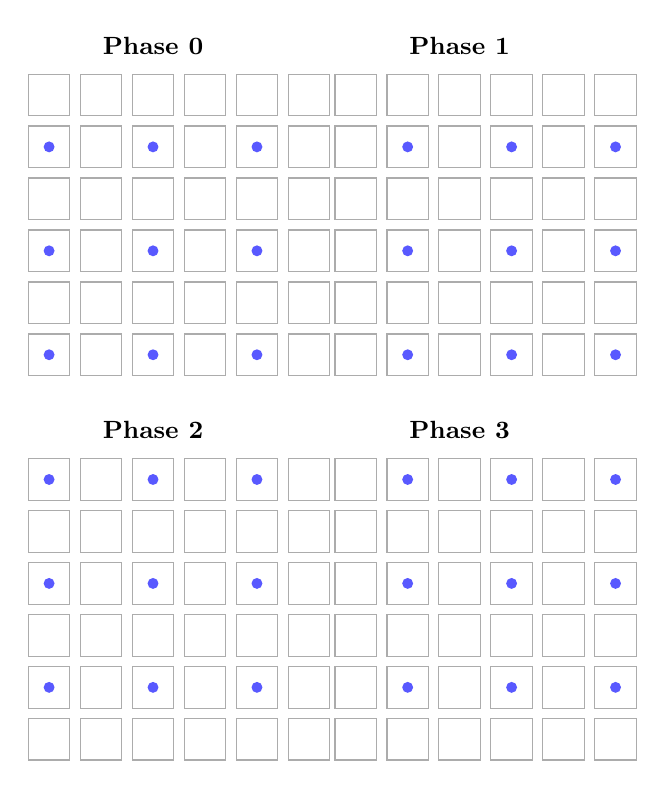
\begin{tikzpicture}[scale=0.66]
\foreach \q/\xo/\yo/\xs/\ys in {
  0/0/0/0/0,
  1/1/0/5.9/0,
  2/0/1/0/-7.4,
  3/1/1/5.9/-7.4
}{
  \begin{scope}[xshift=\xs cm,yshift=\ys cm]
    \node[font=\small\bfseries] at (2.4,6.35) {Phase \q};
    \foreach \i in {0,...,5}{
      \foreach \j in {0,...,5}{
        \draw[gray!65,line width=0.45pt] (\i,\j) rectangle ++(0.8,0.8);
      }
    }
    \foreach \i in {0,2,4}{
      \foreach \j in {0,2,4}{
        \fill[blue!65] ({\i+\xo+0.4},{\j+\yo+0.4}) circle (0.105);
      }
    }
  \end{scope}
}
\end{tikzpicture}
\caption{Four parity-offset step-2 candidate phases. Each panel shows a six-by-six schematic valid-centre grid with one parity class selected at step two. The four phases are alternatives: one is selected for a packet, and only its candidate centres are mutable.}
\label{fig:phases}
\end{figure}

\subsection{Prediction labels and exact reconstruction}

At candidate $i$, the rounded prediction is $p_i$ and the absolute prediction error is $e_i=|X_i-p_i|$. The fixed allocation function maps each $e_i$ to $(n_i,\ell_i,u_i)$, where $n_i$ is the number of MSBs available for replacement and $[\ell_i,u_i]$ is the admissible prediction-error interval used during inverse reconstruction. The 15 distinct triples form the fixed codebook in \cref{tab:codebook}. One four-bit label is stored per candidate. Labels are packed two per byte, high nibble first; the unused low nibble for an odd number of candidates is zero. The packed directory is compressed with zlib level 9 only when the compressed representation is strictly shorter than the raw packed directory.

\begin{table}[t]
\centering
\caption{Fifteen-class allocation codebook used by the proposed system, sorted lexicographically by $(n,\ell,u)$.}
\label{tab:codebook}
\small
\begin{tabular}{rrrr|rrrr}
\toprule
Class & $n$ & $\ell$ & $u$ & Class & $n$ & $\ell$ & $u$\\
\midrule
0 & 0 & 0 & 0 & 8 & 4 & 4 & 4\\
1 & 0 & 64 & 64 & 9 & 4 & 9 & 15\\
2 & 1 & 32 & 32 & 10 & 5 & 2 & 2\\
3 & 1 & 65 & 127 & 11 & 5 & 5 & 7\\
4 & 2 & 16 & 16 & 12 & 6 & 1 & 1\\
5 & 2 & 33 & 63 & 13 & 6 & 3 & 3\\
6 & 3 & 8 & 8 & 14 & 7 & 0 & 0\\
7 & 3 & 17 & 31 & & & &\\
\bottomrule
\end{tabular}
\end{table}

Given the retained low-bit residue $s_i$, prediction $p_i$ and label $(n_i,\ell_i,u_i)$, the decoder searches
\begin{equation}
\mathcal{R}_i=\left\{v\in\{0,\ldots,255\}:
v\bmod 2^{8-n_i}=s_i,\quad
\ell_i\le |v-p_i|\le u_i\right\}.
\label{eq:inverse-set}
\end{equation}
For $n_i>0$, reconstruction is accepted only when $|\mathcal{R}_i|=1$. Candidates with $n_i=0$ are unmodified. The implementation audit exhaustively enumerated all 65,536 original/prediction pairs and 396,032 payload words under positive allocation; it reported zero reconstruction-uniqueness failures and confirmed that the production mapping matched the independently enumerated mapping. This is a finite-domain implementation check, not a general proof for arbitrary future codebooks.

\subsection{In-band packet and cryptographic processing}

The encrypted header is 20 bytes with big-endian layout \texttt{>4sB3sIQ}: a fixed four-byte protocol marker, one-byte codec identifier, three reserved zero bytes, a four-byte directory length $L$, and an eight-byte payload length in bits $P$. The next $L$ candidate bytes store the encrypted packed-label directory, followed by a 32-byte HMAC-SHA256 tag. Thus the bootstrap uses
\begin{equation}
H=20+L+32=52+L
\label{eq:bootstrap}
\end{equation}
candidate bytes. A separate bootstrap-header key and final-header key are derived to avoid reusing a CTR keystream for the two header states.

Let $s$ be the 16-byte big-endian encoding of $V$. The implementation derives $K_{\mathrm{root}}$ from $(K,s)$ using HKDF-SHA256 and derives separate image and data-hiding domains with distinct context strings. Five additional hider keys are derived for bootstrap header, final header, directory, payload and authentication. The image key is not derivable from $\Kh$ under the stated HKDF domain separation. AES-256-CTR is used independently under each derived key with a zero initial counter. Nonce uniqueness under $K$ is mandatory.

The HMAC input binds the image dimensions, the one-byte phase index and the complete row-major marked-image bytes, with the tag-carrier bytes for that phase set to zero before computation. The receiver tests the four public header locations. At each location it decrypts the fixed-size header and validates framing fields and bounds; it then verifies HMAC before directory decryption/decompression or CNN inference. Exactly one phase must pass. Zero or multiple valid phases are rejected. The hider has the authentication key and is therefore trusted to produce valid packets; malicious-hider resistance is not claimed.

\subsection{Signed net-capacity accounting}

Let $C$ be the number of candidates in a phase and $n_i$ the ordinary replaceable bits at candidate $i$. Define gross ordinary slots
\begin{equation}
G_0=\sum_{i=0}^{C-1}n_i.
\end{equation}
The bootstrap occupies $H=52+L$ candidate bytes. The ordinary slots forgone at those carrier candidates are
\begin{equation}
F=\sum_{i=0}^{H-1}n_i.
\end{equation}
The remaining ordinary stream contains $S=G_0-F$ bits. To restore the original $H$ bootstrap candidate bytes, the owner preserves $B=8H$ bits in the ordinary stream. The signed net user-payload budget is
\begin{equation}
N_{\mathrm{net}}=S-B=G_0-F-8H.
\label{eq:net}
\end{equation}
An image is rejected if $N_{\mathrm{net}}\le0$. We report signed net rate $N_{\mathrm{net}}/(HW)$ and usable net rate $\max(0,N_{\mathrm{net}})/(HW)$.

The physical metadata occupies $8H$ bits in the bootstrap. Its opportunity cost in ordinary carrier slots is $F$, because the first $H$ candidates no longer supply their usual $n_i$ bits. The bootstrap backup is the separate cost $B=8H$. The ledger reports physical metadata storage, foregone ordinary slots and backup bits separately. The physical metadata storage is not subtracted a second time from \cref{eq:net}; doing so would double-count the same bootstrap region.

For each phase $q$, the owner independently recomputes predictions, labels, compressed directory, $H_q$, $F_q$ and $N_q$, and selects
\begin{equation}
q^\star=\arg\max_{q\in\{0,1,2,3\}}N_q,
\label{eq:phase-select}
\end{equation}
using the lowest phase index to break ties. The image is rejected if $\max_qN_q\le0$.

\begin{figure}[t]
\centering
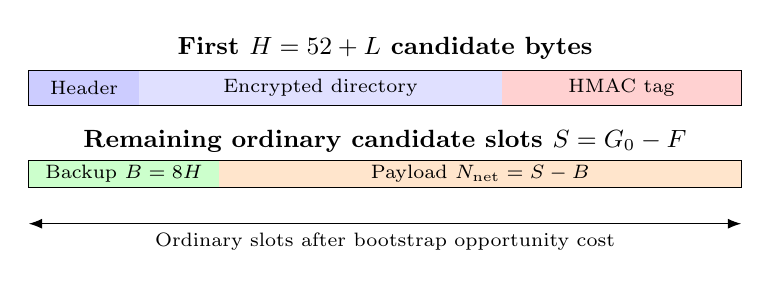
\begin{tikzpicture}[x=0.78cm,y=0.72cm,>=Latex]
  \node[font=\small\bfseries] at (5.8,3.0) {First $H=52+L$ candidate bytes};
  \draw[thick] (0,2) rectangle (11.6,2.6);
  \fill[blue!20] (0,2) rectangle (1.8,2.6);
  \fill[blue!12] (1.8,2) rectangle (7.7,2.6);
  \fill[red!18] (7.7,2) rectangle (11.6,2.6);
  \node[font=\scriptsize] at (0.9,2.3) {Header};
  \node[font=\scriptsize] at (4.75,2.3) {Encrypted directory};
  \node[font=\scriptsize] at (9.65,2.3) {HMAC tag};
  \node[font=\small\bfseries] at (5.8,1.35) {Remaining ordinary candidate slots $S=G_0-F$};
  \draw[thick] (0,0.55) rectangle (11.6,1.0);
  \fill[green!20] (0,0.55) rectangle (3.1,1.0);
  \fill[orange!20] (3.1,0.55) rectangle (11.6,1.0);
  \node[font=\scriptsize] at (1.55,0.78) {Backup $B=8H$};
  \node[font=\scriptsize] at (7.35,0.78) {Payload $N_{\mathrm{net}}=S-B$};
  \draw[<->] (0,-0.1) -- (11.6,-0.1);
  \node[below,font=\scriptsize] at (5.8,-0.1) {Ordinary slots after bootstrap opportunity cost};
\end{tikzpicture}
\caption{Schematic packet and signed-net accounting. The bootstrap occupies $8H$ physical metadata bits; it forfeits $F$ ordinary replacement bits at the bootstrap candidates. The original bootstrap bytes are restored using a separate $B=8H$-bit prefix of the remaining ordinary stream.}
\label{fig:packet}
\end{figure}

\subsection{Owner, hider and receiver procedure}

The owner validates native uint8 grayscale mode and even image dimensions; evaluates all four phases separately; builds and losslessly codes each label directory; chooses the maximum signed net phase; saves the original bootstrap bytes in the backup prefix; writes zero reservation bits; encrypts the reserved image; and installs the encrypted bootstrap header, directory and HMAC tag. The owner has no user-payload argument during reservation.

The hider authenticates the bootstrap packet, decrypts and validates the bounded directory, reconstructs the ordinary slot stream, checks that the payload length does not exceed the reserved net capacity, encrypts the padded payload under its dedicated subkey, writes ciphertext bits into the reserved ordinary slots, and replaces the bootstrap header with the final payload length and recomputed HMAC. The hider does not decrypt the image or require the CNN.

The receiver derives its keys from $(K,V)$, tests the four possible final-header locations, accepts exactly one authenticated and bounded directory, extracts and decrypts payload bits, checks payload padding, restores the known-zero reservation positions before image decryption, reconstructs candidate pixels using \cref{eq:inverse-set}, restores the original bootstrap bytes from the backup prefix and returns both host and payload. The receiver process uses the marked image as its only per-image data file.

\begin{figure}[t]
\centering
\resizebox{\textwidth}{!}{%
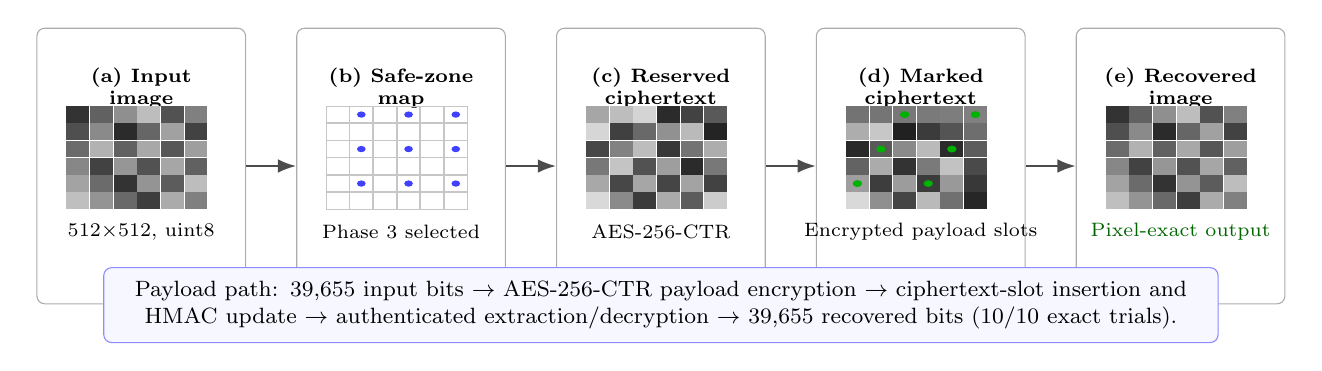
\begin{tikzpicture}[x=1.0cm,y=0.73cm,>=Latex,
  frame/.style={draw=gray!65,rounded corners=1mm,minimum width=2.65cm,minimum height=3.5cm,align=center},
  title/.style={font=\scriptsize\bfseries,text width=2.65cm,align=center},
  arrow/.style={->,thick,draw=black!70}]
% Original schematic host tile.
\node[frame] (orig) at (1.35,0) {};
\node[title] at (1.35,1.35) {(a) Input\\image};
\foreach \i in {0,...,5}{\foreach \j in {0,...,5}{
  \pgfmathtruncatemacro{\shade}{25+mod(17*\i+11*\j+5*\i*\j,60)}
  \fill[black!\shade] ({0.4+0.30*\i},{-0.75+0.30*\j}) rectangle ++(0.29,0.29);
}}
\node[font=\scriptsize,align=center] at (1.35,-1.15) {512$\times$512, uint8};
% Safe-zone grid, q=3.
\node[frame] (safe) at (4.65,0) {};
\node[title] at (4.65,1.35) {(b) Safe-zone\\map};
\foreach \i in {0,...,5}{\foreach \j in {0,...,5}{
  \draw[gray!45,line width=0.35pt] ({3.70+0.30*\i},{-0.75+0.30*\j}) rectangle ++(0.29,0.29);
}}
\foreach \i in {1,3,5}{\foreach \j in {1,3,5}{
  \fill[blue!75] ({3.70+0.30*\i+0.145},{-0.75+0.30*\j+0.145}) circle (0.055);
}}
\node[font=\scriptsize,align=center] at (4.65,-1.15) {Phase 3 selected};
% Reserved ciphertext schematic.
\node[frame] (cipher) at (7.95,0) {};
\node[title] at (7.95,1.35) {(c) Reserved\\ciphertext};
\foreach \i in {0,...,5}{\foreach \j in {0,...,5}{
  \pgfmathtruncatemacro{\shade}{15+mod(31*\i+19*\j+7*\i*\j,75)}
  \fill[black!\shade] ({7.00+0.30*\i},{-0.75+0.30*\j}) rectangle ++(0.29,0.29);
}}
\node[font=\scriptsize,align=center] at (7.95,-1.15) {AES-256-CTR};
% Marked ciphertext schematic.
\node[frame] (marked) at (11.25,0) {};
\node[title] at (11.25,1.35) {(d) Marked\\ciphertext};
\foreach \i in {0,...,5}{\foreach \j in {0,...,5}{
  \pgfmathtruncatemacro{\shade}{15+mod(29*\i+23*\j+9*\i*\j,75)}
  \fill[black!\shade] ({10.30+0.30*\i},{-0.75+0.30*\j}) rectangle ++(0.29,0.29);
}}
\foreach \i/\j in {0/1,1/3,2/5,3/1,4/3,5/5}{
  \fill[green!70!black] ({10.30+0.30*\i+0.145},{-0.75+0.30*\j+0.145}) circle (0.06);
}
\node[font=\scriptsize,align=center] at (11.25,-1.15) {Encrypted payload slots};
% Recovered schematic host tile, same representation as the input tile.
\node[frame] (recovered) at (14.55,0) {};
\node[title] at (14.55,1.35) {(e) Recovered\\image};
\foreach \i in {0,...,5}{\foreach \j in {0,...,5}{
  \pgfmathtruncatemacro{\shade}{25+mod(17*\i+11*\j+5*\i*\j,60)}
  \fill[black!\shade] ({13.60+0.30*\i},{-0.75+0.30*\j}) rectangle ++(0.29,0.29);
}}
\node[font=\scriptsize,align=center,text=green!40!black] at (14.55,-1.15) {Pixel-exact output};
\draw[arrow] (orig.east) -- (safe.west);
\draw[arrow] (safe.east) -- (cipher.west);
\draw[arrow] (cipher.east) -- (marked.west);
\draw[arrow] (marked.east) -- (recovered.west);
\node[draw=blue!45,fill=blue!3,rounded corners=1mm,text width=13.8cm,align=center,font=\footnotesize,inner sep=5pt] at (7.95,-2.42)
{Payload path: 39,655 input bits $\rightarrow$ AES-256-CTR payload encryption $\rightarrow$ ciphertext-slot insertion and HMAC update $\rightarrow$ authenticated extraction/decryption $\rightarrow$ 39,655 recovered bits (10/10 exact trials).};
\end{tikzpicture}%
}
\caption{Schematic view of the evaluated end-to-end stages. The phase-3 lattice is the selected phase in the ten-repeat $512\times512$ benchmark. The grayscale tiles and ciphertext textures are illustrative diagrams, not raw image or ciphertext dumps; measured stage timings and exact-recovery outcomes are reported in Table~\ref{tab:e2e-stage}.}
\label{fig:e2e-stages}
\end{figure}


\section{Experimental design}
\label{sec:experiments}

\subsection{Corpus and curation}

The evaluation corpus contains 243 distinct native 8-bit grayscale USC-SIPI images. The final curation labels 232 images as natural-labelled and 11 as constructed texture mosaics. Two source files with duplicate decoded pixel arrays were removed from 245 catalogue-curated inputs; five nonconforming files were skipped. Images were read in native mode L without resizing, cropping, colour conversion or recompression. The dimensions were 256$\times$256 for 62 images, 512$\times$512 for 152 images and 1024$\times$1024 for 29 images. The image ledger contains 29 provenance/correlation clusters. The 232 natural-labelled cases include sequences and rotated texture series; they should not be interpreted as 232 independent natural photographs.

The final evaluation manifest records the six canonical small-image baseline stems (Airplane, Baboon, Goldhill, Jetplane, Lena and Peppers) as absent from this expanded corpus. Accordingly, the paper does not claim that these six classic images are part of the 243-image evaluation. Per-file source SHA-256 and decoded-pixel SHA-256 values were retained for all 243 accepted images.

\begin{table}[t]
\centering
\caption{Final grayscale corpus composition.}
\label{tab:corpus}
\small
\begin{tabular}{lrr}
\toprule
Stratum & Images & Percentage\\
\midrule
Natural-labelled & 232 & 95.47\\
Constructed texture mosaics & 11 & 4.53\\
\midrule
Total & 243 & 100.00\\
\addlinespace
$256\times256$ & 62 & 25.51\\
$512\times512$ & 152 & 62.55\\
$1024\times1024$ & 29 & 11.93\\
\bottomrule
\end{tabular}
\end{table}

\subsection{Evaluation protocol and estimands}

All final evaluations used frozen checkpoints; no training or fine-tuning was performed during the evaluation runs. The active CNN-3$\times$3 checkpoint SHA-256 and model architecture are reported in \cref{sec:method}. The training corpus, source-image inventory, train/validation split, random seed and full checkpoint-selection history were not available in the final evaluation artifacts. The manuscript therefore does not claim that training/test leakage has been independently excluded; this provenance must be supplied before submission.

For image $j$, let $N_j$ be its signed net payload and $P_j=H_jW_j$ its pixel count. The paper reports (i) positive-net coverage, (ii) all-image mean signed rate, (iii) mean usable rate with rejected images set to zero, (iv) pooled usable rate $\sum_j\max(0,N_j)/\sum_jP_j$, and (v) the median and quartiles of per-image usable rates. Positive-only averages are not used as the primary capacity claim. Uncertainty is estimated by cluster bootstrap over the 29 provenance/correlation clusters with 10,000 replicates and seed 20261119. The reported intervals are descriptive for this corpus; they do not eliminate dataset-selection or training-provenance limitations.

\subsection{Predictor comparison}

The predictor-only comparison uses a common step-4 grid with 16 phases and a three-pixel border so that the largest tested $7\times7$ predictor and classical predictors use the same candidate positions. This experiment evaluates prediction MAE and positive-net coverage under a shared comparison grid. It is separate from the native implementation, which uses its step-2/four-phase grid. The CALIC reference is a simplified CALIC-style predictor, not a full canonical CALIC implementation. The compared learned models are frozen checkpoints; the $5\times5$ no-weighted-loss model is included as an ablation.

\subsection{External native-protocol replications}

Multi-MSB+Huffman and PPMR were reproduced on the same 243 decoded source images and pixel arrays as \ProposedSystem. The Multi-MSB+Huffman evaluation adapter passes the actual embedded payload count reported by the source method to its extractor. PPMR required four narrow compatibility repairs in a temporary copy: two repairs to the bit-plane 7/8 encoder/decoder branch structure and two active-plane extraction-order corrections. The results are therefore labelled corrected PPMR, not an unmodified upstream run. The reproduction used GNU Octave on Linux; equivalence of Octave and MATLAB random-number streams is not claimed.

The paired comparison checks exact source-file and decoded-pixel hashes. The final merge contains 243 unique image IDs, no missing or duplicate rows, and 243 exact image and payload passes for both external methods. Rates remain each method's native protocol rates. This is a matched-corpus comparison, not identical carrier geometry, packet cost, encryption order, authentication or receiver-side-information assumptions.

\subsection{Correctness, security tests and runtime}

The grayscale evaluation ledger records six payload cases for each positive-net image: empty, one-bit, short, partial, near-maximum and full measured-capacity. The total is $163\times6=978$ receiver trials. Image and payload equality are checked independently.

The finite-domain mapping audit enumerates all 65,536 prediction/original pairs and 396,032 valid payload words under positive allocations. A 20,000-input Atheris parser-fuzz campaign reports zero crashes, with 121 coverage counters and 188 feature counters. Deterministic malformed-packet and mutation tests additionally exercise header bounds, reserved bytes, directory codec/length handling, authentication failures, wrong key/nonce cases and bounded compressed-directory rejection. These are implementation robustness tests, not a formal cryptographic proof.

Two performance measurements have different scopes and are kept separate. The predictor-only benchmark used a deterministic synthetic $512\times512$ grayscale image, five warm-up runs and ten CPU repeats with four PyTorch threads. The later E2E benchmark used USC-SIPI image 5.2.08.tiff, two warm-ups and ten measured CPU repetitions with the model resident, two threads and vectorised patch extraction. The optimisation was checked against the original patch-extraction path and produced identical patch arrays and zero rounded-prediction mismatches under the validated settings. The E2E benchmark excludes process startup, checkpoint loading, file I/O and dataset acquisition. RSS was sampled every 5 ms, so short-lived peaks may be missed.

\section{Results}
\label{sec:results}

\subsection{Native grayscale capacity and exact recovery}

The native grayscale results are summarised in Tables~\ref{tab:capacity} and~\ref{tab:overhead}. Positive net capacity was achieved on 163 of 243 images. All 978 receiver trials on this accepted subset recovered both the host image and payload exactly; the six payload cases and robustness coverage are listed in Table~\ref{tab:robustness}.

\begin{table}[t]
\centering
\caption{Implementation correctness and parser-robustness evidence. Results are finite implementation tests, not formal security proofs.}
\label{tab:robustness}
\scriptsize
\begin{tabularx}{\textwidth}{p{3.0cm}p{7.5cm}X}
\toprule
Test family & Coverage & Result\\
\midrule
Finite inverse-map enumeration & 65,536 original/prediction pairs; 396,032 positive-allocation payload words. & Zero mapping failures.\\
Full-corpus receiver tests & Six payload sizes for each of 163 positive-net images. & 978/978 exact host and payload recoveries.\\
Phase/header discovery & Four candidate header locations; framing, bounds, phase-bound authentication and ambiguity checks. & Regression tests passed.\\
Mutation and malformed-packet tests & Wrong keys/nonces; header, directory, tag and payload changes; malformed fields and lengths. & Covered cases rejected or parsed within bounds.\\
Coverage-guided parser fuzzing & 20,000 Atheris inputs. & Zero crashes; 121 coverage and 188 feature counters.\\
\bottomrule
\end{tabularx}
\end{table}

\begin{table}[t]
\centering
\caption{Net-capacity results over the full 243-image corpus.}
\label{tab:capacity}
\small
\begin{tabular}{lr}
\toprule
Metric & Result\\
\midrule
Images & 243\\
Positive-net images & 163/243 (67.08\%)\\
Non-positive images & 80/243\\
Mean signed net rate (all images) & 0.11054 bpp\\
Mean usable rate (all images, rejected set to zero) & 0.14322 bpp\\
Pooled usable rate & 0.09550 bpp\\
Median usable rate & 0.04705 bpp\\
First / third quartile & 0.00000 / 0.19497 bpp\\
95\% CI: mean usable rate (29-cluster bootstrap) & [0.06139, 0.25038] bpp\\
95\% CI: positive-net coverage & [50.19\%, 82.39\%]\\
Exact image-and-payload trials & 978/978\\
\bottomrule
\end{tabular}
\end{table}

\subsection{Capacity heterogeneity across image strata}

The stratified outcomes are given in Tables~\ref{tab:resolution} and~\ref{tab:classification}. Differences across strata reflect both image content and directory/bootstrap costs; they should not be interpreted as a controlled resolution or natural-versus-constructed experiment.


\begin{table}[t]
\centering
\caption{Mean bootstrap and carrier-cost decomposition over all 243 images. Per-image rates are arithmetic means; pooled rates divide total bits by total pixels. Metadata wire storage is descriptive and is not subtracted a second time in the net equation.}
\label{tab:overhead}
\scriptsize
\begin{tabularx}{\textwidth}{Xrrr}
\toprule
Quantity & Mean bits / image & Mean rate (bpp) & Pooled (bpp)\\
\midrule
Gross ordinary carrier slots $G_0$ & 383,672 & 1.28949 & 1.25451\\
Bootstrap opportunity cost $F$ & 140,541 & 0.46177 & 0.45953\\
Physical in-band metadata storage $8H$ & 224,836 & 0.71718 & 0.73515\\
Original bootstrap-byte backup $B=8H$ & 224,836 & 0.71718 & 0.73515\\
Total charged overhead $F+B$ & 365,377 & 1.17895 & 1.19469\\
\midrule
Signed net payload $N_{\mathrm{net}}$ & 18,295 & 0.11054 & 0.05982\\
\bottomrule
\end{tabularx}
\end{table}

\begin{table}[t]
\centering
\caption{Capacity by image dimension. Mean usable rate is the arithmetic per-image mean; pooled usable rate divides total usable bits by total pixels.}
\label{tab:resolution}
\small
\begin{tabular}{lrrrr}
\toprule
Resolution & Images & Positive & Coverage & Mean / pooled usable bpp\\
\midrule
$256\times256$ & 62 & 45 & 72.58\% & 0.19549 / 0.19549\\
$512\times512$ & 152 & 108 & 71.05\% & 0.14624 / 0.14624\\
$1024\times1024$ & 29 & 10 & 34.48\% & 0.01564 / 0.01564\\
\bottomrule
\end{tabular}
\end{table}

\begin{table}[t]
\centering
\caption{Capacity by final curation label.}
\label{tab:classification}
\small
\begin{tabular}{lrrrr}
\toprule
Curation label & Images & Positive & Coverage & Mean usable bpp\\
\midrule
Natural-labelled & 232 & 159 & 68.53\% & 0.14902\\
Constructed texture mosaics & 11 & 4 & 36.36\% & 0.02088\\
\bottomrule
\end{tabular}
\end{table}

\subsection{Effect of four-phase selection}

Table~\ref{tab:phases} and Figure~\ref{fig:phase-results} summarise fixed-phase and adaptive selection. Adaptive selection never reduced the signed net budget relative to Phase~0, but increased positive-net coverage by only two images.

\begin{table}[t]
\centering
\caption{Fixed-phase and adaptive phase-selection outcomes.}
\label{tab:phases}
\small
\begin{tabularx}{\textwidth}{Xrrr}
\toprule
Selection & Positive & Signed bpp & Usable bpp\\
\midrule
Fixed phase 0 & 161/243 & 0.10735 & 0.14070\\
Fixed phase 1 & 158/243 & 0.10311 & 0.13709\\
Fixed phase 2 & 161/243 & 0.10917 & 0.14231\\
Fixed phase 3 & 159/243 & 0.10624 & 0.13981\\
Adaptive max-net & 163/243 & 0.11054 & 0.14322\\
\bottomrule
\end{tabularx}
\end{table}

\begin{figure}[t]
\centering
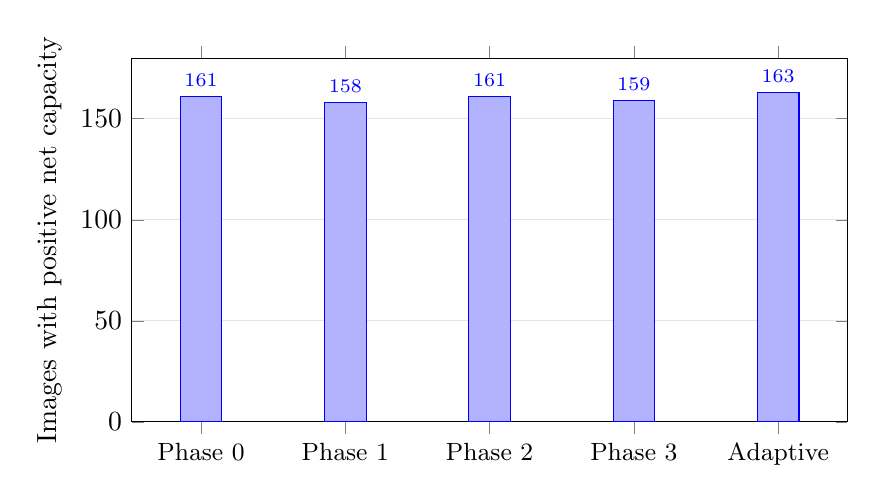
\begin{tikzpicture}
\begin{axis}[
  ybar,
  width=0.88\textwidth,height=6.2cm,
  ymin=0,ymax=180,
  ylabel={Images with positive net capacity},
  symbolic x coords={Phase 0,Phase 1,Phase 2,Phase 3,Adaptive},
  xtick=data,
  x tick label style={font=\small},
  nodes near coords,
  nodes near coords style={font=\scriptsize},
  bar width=15pt,
  enlarge x limits=0.12,
  ymajorgrids=true,
  grid style={gray!20}
]
\addplot coordinates {(Phase 0,161) (Phase 1,158) (Phase 2,161) (Phase 3,159) (Adaptive,163)};
\end{axis}
\end{tikzpicture}
\caption{Positive-net coverage for each fixed phase and the adaptive four-phase choice. Adaptive selection increases coverage by two images relative to phase 0.}
\label{fig:phase-results}
\end{figure}

\subsection{Matched-grid predictor comparison}

Table~\ref{tab:predictors} and Figure~\ref{fig:predictor} report the matched-grid predictor study. This step-4/16-phase experiment is separate from native EDR2. The selected CNN-3$\times$3 is retained for its radius-one synchronization geometry, not because it is the best predictor; the $5\times5$ no-weighted-loss ablation performs better on both reported measures.

\begin{table}[t]
\centering
\caption{Predictor comparison on a common step-4/16-phase grid. Positive-net outcomes and MAE are measured within this separate predictor study; they are not native step-2/four-phase capacity results.}
\label{tab:predictors}
\small
\begin{tabular}{lrrr}
\toprule
Predictor & Mean candidate MAE & Positive-net images & Coverage\\
\midrule
MED & 7.9503 & 49/243 & 20.16\%\\
GAP & 7.8408 & 58/243 & 23.87\%\\
Simplified CALIC-style & 8.2021 & 49/243 & 20.16\%\\
CNN-5$\times$5 residual & 4.6324 & 138/243 & 56.79\%\\
CNN-5$\times$5 no residual & 4.6573 & 139/243 & 57.20\%\\
CNN-5$\times$5 no weighted loss & 4.6233 & 140/243 & 57.61\%\\
CNN-3$\times$3 checkpoint & 4.8130 & 133/243 & 54.73\%\\
CNN-7$\times$7 residual & 4.6882 & 140/243 & 57.61\%\\
\bottomrule
\end{tabular}
\end{table}

\begin{figure}[t]
\centering
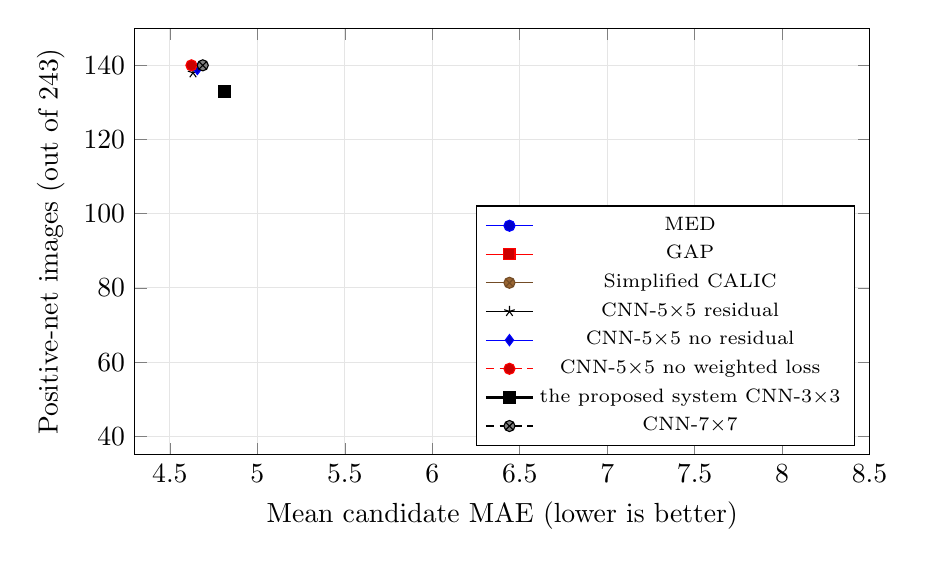
\begin{tikzpicture}
\begin{axis}[
  width=0.9\textwidth,height=7.0cm,
  xlabel={Mean candidate MAE (lower is better)},
  ylabel={Positive-net images (out of 243)},
  xmin=4.3,xmax=8.5,ymin=35,ymax=150,
  grid=both,grid style={gray!20},
  legend style={at={(0.98,0.02)},anchor=south east,font=\scriptsize},
  every axis plot/.append style={mark=*}
]
\addplot coordinates {(7.9503,49)};\addlegendentry{MED}
\addplot coordinates {(7.8408,58)};\addlegendentry{GAP}
\addplot coordinates {(8.2021,49)};\addlegendentry{Simplified CALIC}
\addplot coordinates {(4.6324,138)};\addlegendentry{CNN-5$\times$5 residual}
\addplot coordinates {(4.6573,139)};\addlegendentry{CNN-5$\times$5 no residual}
\addplot coordinates {(4.6233,140)};\addlegendentry{CNN-5$\times$5 no weighted loss}
\addplot[mark=square*,thick] coordinates {(4.8130,133)};\addlegendentry{the proposed system CNN-3$\times$3}
\addplot coordinates {(4.6882,140)};\addlegendentry{CNN-7$\times$7}
\end{axis}
\end{tikzpicture}
\caption{Predictor MAE against positive-net outcomes under the common step-4 comparison grid. The proposed CNN-3$\times$3 model is highlighted; the 5$\times$5 no-weighted-loss ablation is better on both reported measures.}
\label{fig:predictor}
\end{figure}

\subsection{Same-corpus native-protocol external comparison}

The complete-method comparison is in Table~\ref{tab:external}. All methods were evaluated on the same 243 source/pixel records, but each retains its native carrier, metadata accounting and security assumptions; the rates are therefore not an identical-packet-cost leaderboard.

\begin{table}[t]
\centering
\caption{Paired same-corpus native-protocol results over 243 hash-matched images. Each method retains its native carrier and overhead expression; rates are not a same-packet-cost or same-security-model leaderboard.}
\label{tab:external}
\scriptsize
\setlength{\tabcolsep}{4pt}
\begin{tabular}{p{4.7cm}>{\centering\arraybackslash}p{1.45cm}>{\centering\arraybackslash}p{1.85cm}>{\centering\arraybackslash}p{1.85cm}>{\centering\arraybackslash}p{2.15cm}}
\toprule
Method & Positive images & Mean usable (bpp) & Pooled usable (bpp) & Exact recovery\\
\midrule
Proposed system, step-2/four-phase & 163/243 & 0.14322 & 0.09550 & 978/978 accepted\\
Multi-MSB+Huffman & 243/243 & 2.08848 & 1.97350 & 243/243\\
Corrected PPMR & 238/243 & 2.22817 & 2.11817 & 243/243\\
\bottomrule
\end{tabular}
\end{table}

All three methods passed the image/payload equality checks recorded in the comparison ledger. The PPMR result is labelled as corrected because four compatibility repairs were applied in a temporary checkout; the upstream repository was not modified.

\subsection{Runtime and memory}

Table~\ref{tab:runtime} separates the predictor-only comparison from the optimised end-to-end measurement. The latter is a single-image, warmed CPU benchmark; Table~\ref{tab:e2e-stage} details the observed safe-zone choice, encryption, encrypted-domain embedding, receiver stages and exact outputs. The two timing scopes should not be treated as one benchmark series.

\begin{table}[t]
\centering
\caption{Runtime and model-complexity summary. Predictor-only and end-to-end measurements use different scopes.}
\label{tab:runtime}
\scriptsize
\begin{tabularx}{\textwidth}{p{2.65cm}p{4.0cm}X}
\toprule
Measurement & Measured value & Protocol note\\
\midrule
MED predictor & 3.826 ms mean & Synthetic $512\times512$ input; four CPU threads; predictor-only.\\
CNN-$3\times3$ predictor & 708.479 ms mean & Same predictor-only harness; 185.2$\times$ the MED time.\\
CNN-$3\times3$ model & 46,881 parameters; 122,816 MAC/patch & Conv2d and Linear operations; non-matrix operations excluded.\\
Four-phase lattice & 7.986B MAC/phase; 31.944B MAC/four phases & 65,025 candidate patches per phase on a $512\times512$ image; operation-count estimate.\\
Optimised E2E & 1.1140 s mean; SD 0.0581 s; median 1.1204 s & One native $512\times512$ image; two warm-ups, ten measured repeats; model resident.\\
E2E memory & +10.87 MiB sampled RSS & RSS sampled every 5 ms; transient peaks may be missed.\\
\bottomrule
\end{tabularx}
\end{table}

\begin{table}[t]
\centering
\caption{Measured end-to-end outcomes for USC-SIPI image 5.2.08.tiff ($512\times512$). Ten warmed CPU repetitions used full measured capacity and distinct benchmark nonces.}
\label{tab:e2e-stage}
\scriptsize
\begin{tabularx}{\textwidth}{p{3.05cm}X>{\centering\arraybackslash}p{2.15cm}}
\toprule
Stage & Measured output & Time / result\\
\midrule
Safe-zone mapping & Phase 3 selected in all ten runs; 65,025 candidate centres per phase (24.81\% of pixels). & 10/10 phase 3\\
Prepare + directory & Frozen CNN-$3\times3$ generated predictions, allocation labels and compressed directory. & 0.5823 s\\
Reserve + encrypt & Bootstrap and original-byte backup reserved; image encrypted with AES-256-CTR. & 0.0702 s\\
Ciphertext embedding & 39,655 payload bits (0.151272 bpp) inserted; final header and HMAC updated. & 0.0433 s\\
Receiver & Packet authenticated; payload extracted/decrypted and host reconstructed. & 0.4183 s\\
Recovered image & Pixel-wise equality with the source image. & 10/10 exact\\
Recovered payload & Bit-wise equality with the 39,655-bit input payload. & 10/10 exact\\
\midrule
Total pipeline & Mean 1.1140 s; SD 0.0581 s; median 1.1204 s. Sampled RSS increased by 10.87 MiB. & 1.1140 s\\
\bottomrule
\end{tabularx}
\end{table}

\section{Security analysis}
\label{sec:security}

\subsection{Implementation verification}
The implementation checks cover finite-domain inverse-map enumeration, the accepted-image round trips, authenticated phase discovery, malformed-packet and mutation cases, and a 20,000-input parser-fuzz campaign. Their tested scope and outcomes are summarised in Table~\ref{tab:robustness}; they are implementation evidence for the covered cases.

\subsection{Cryptographic interpretation}

HKDF context separation prevents accidental reuse of one derived key across image encryption, staged headers, directory, payload and authentication. AES-256-CTR provides confidentiality only under the required unique-key/nonce discipline; it is malleable and is not treated as an integrity mechanism. The implementation uses the standard CTR mode and HMAC construction, with per-domain keys derived through HKDF-SHA256 \cite{nist2001,rfc2104,rfc5869}. The HMAC-SHA256 tag authenticates the marked packet against parties lacking the authentication key. Since the authorised hider has that key, it can recompute a valid tag after changing the packet; the protocol therefore trusts the hider. The owner-to-hider key handoff is assumed confidential and authenticated. No formal cryptographic reduction, side-channel analysis, nonce-misuse test suite or independent cryptographic audit is claimed.

\subsection{Scope and limitations}

The principal limitations are grouped into three areas. First, net payload remains below the two reproduced external methods, and only 163 of 243 images carry positive net capacity; the external comparison uses native protocol accounting rather than identical packet and security assumptions. Second, the CNN-$3\times3$ choice is a synchronization-geometry and model-size trade-off, not a predictor-accuracy claim: the $5\times5$ no-weighted-loss ablation performs better in the separate matched-grid study, while the selected CNN is slower than MED in the predictor-only CPU benchmark. Third, the evaluated protocol is limited to even-sized native 8-bit grayscale images. The frozen checkpoint's complete training provenance and an independent cryptographic review remain outstanding; the reported tests establish implementation behaviour for the tested cases, not a formal security proof.

The system falls within multimedia security, but its strongest possible JISA argument is the concrete connection between a local predictor's receptive field, a deterministic carrier geometry, authenticated in-band phase discovery and a receiver-side recovery contract. Elsevier describes JISA as a journal for original, practice-driven information-security research and explicitly lists multimedia security and forensics among its topics. Its journal description also cautions against formal-only work without implementation or empirical testing, and routine AI/ML applications without a substantial security contribution \cite{jisaScope}. the implementation includes empirical validation, but the current results do not show high payload capacity and the narrow novelty may be judged incremental beside recent JISA methods. A submission should be attempted only if the authors can complete the checkpoint training provenance, strengthen the prior-art distinction with full-text review, and defend why the synchronization property constitutes a nontrivial security/engineering contribution despite the payload gap. The present manuscript does not recommend a high-capacity or state-of-the-art framing.

\section{Conclusion}
\label{sec:conclusion}

This paper presented the proposed system, an RRBE protocol that combines a centre-masked CNN-$3\times3$, four maximum-density step-2 phases, maximum signed-net phase selection and authenticated in-band phase discovery. The formal result establishes that writes to one selected phase cannot alter any candidate's masked radius-one predictor input. The implementation and evaluation connect this geometry to a receiver-side recovery contract without image-dependent sidecar maps.

The 243-image evaluation, phase ablation, predictor study, external native-protocol comparison and end-to-end stage measurements are summarised in Tables~\ref{tab:capacity}--\ref{tab:e2e-stage} and Figures~\ref{fig:system-overview}--\ref{fig:predictor}. The evidence demonstrates exact recovery for every tested accepted-case trial, while showing that usable capacity is lower than the two reproduced methods and that the chosen $3\times3$ checkpoint is not the strongest predictor in the matched-grid ablation. The contribution is therefore the specific synchronization and authenticated packet/recovery construction, not capacity or predictor superiority.

\section*{Data availability}
The evaluation uses hash-pinned source and decoded-pixel manifests, a per-image capacity ledger, exact-recovery records, baseline comparison tables, runtime evidence and parser-test evidence archived with the project repository. Add a persistent release/DOI for the final source and supplement before submission; a GitHub Actions artifact alone should not be treated as a permanent archival repository.

\section*{Funding}
[Insert funding information or state that no specific funding was received, if accurate.]

\section*{Acknowledgements}
[Insert acknowledgements or remove this section.]

\bibliographystyle{elsarticle-num}
\bibliography{EDR2_JISA_References}

\end{document}
